\documentclass[12pt]{article}
\setlength{\parindent}{0pt}
\usepackage{amsmath, amssymb, geometry,esint}
\usepackage{graphicx}
\usepackage{multicol, paracol}
\usepackage{pdfpages}
\geometry{a4paper, margin=0.1in}
\title{Electromagnetics 1 Final Formula Sheet}
\author{SalahDin Rezk}
\date{\today}
\begin{document}
\begin{multicols}{3}
  \textbf{Coulomb's Law}: $\mathbf{F} = \frac{1}{4 \pi \epsilon_0} \frac{q_1 q_2}{|\mathbf{r}|^2} \hat{\mathbf{r}}$ \\
  \textbf{Electric Field}: $\mathbf{E} = \frac{1}{4 \pi \epsilon_0} \frac{q}{|\mathbf{r}|^2} \hat{\mathbf{r}}$ \\
  \textbf{Gauss's Law}: $\oint \mathbf{E} \cdot d\mathbf{A} = \frac{Q_{\text{enc}}}{\epsilon_0}$ \\
  \textbf{Electric Potential}: $V = - \int \mathbf{E} \cdot d\mathbf{l}$ \\
  \textbf{$\mathbf{E}$ and $V$}: $\mathbf{E} = -\nabla V$ \\
  \textbf{Laplace's Equation}: $\nabla^2 V = 0$ \\
  \textbf{Poisson's Equation}: $\nabla^2 V = -\frac{\rho_v}{\epsilon}$ \\
  \textbf{Work Done}: $W=-Q\int_{a}^{b} \mathbf{E} \cdot d\mathbf{l}$\\
  \textbf{$V$ and $W$}: $V_{ba}=\frac{W_{ba}}{Q}$\\
  \textbf{Electric Displacement}: $\mathbf{D} = \epsilon\mathbf{E}$ \\
  \textbf{Current Density}: $\mathbf{J} = \sigma \mathbf{E}$ \\
  \textbf{Continuity Eq}: $\nabla \cdot \mathbf{J} = -\partial_{t} \rho_v$ \\
  \textbf{Current}: $I = \frac{dQ}{dt}$ \\
  \textbf{Total Current}: $I = \iint_S \mathbf{J} \cdot d\mathbf{A}$ \\
  \textbf{Ohm's Law}: $V = IR$ \\
  \textbf{Capacitance}: $C = \frac{Q}{V} = \iint_S \frac{1}{\int_L \frac{dL_{\parallel}}{\epsilon dS_{\perp}}}$ \\
  \textbf{Parallel Plate Capacitor}: $C = \frac{\epsilon A}{d}$ \\
  \textbf{Current in Capacitor}: $I = C \frac{dV}{dt}$ \\
  \textbf{Capacitor Energy}: $U = \frac{1}{2} C V^2$ \\
  \textbf{Capacitor Electric Field}: $E = \frac{V}{d}$ \\
  \textbf{Work}: $W=QV=\frac{CV^2}{2}=\frac{QV}{2}=\frac{Q^2}{2C}$\\
  \textbf{Work Density}: $W_E=\frac{P_{v}V}{2}=\frac{D^2}{2\epsilon}$\\
  \textbf{Biot-Savart Law}: $\mathbf{B} = \frac{\mu_0}{4 \pi} \int \frac{I d\mathbf{l} \times \hat{\mathbf{r}}}{|\mathbf{r}|^2}$ \\
  \textbf{Ampere's Law}: $\oint \mathbf{H} \cdot d\mathbf{l} = I_{\text{enc}}$ \\
  \textbf{Magnetic Flux Density}: $\mathbf{B} = \mu \mathbf{H}$ \\
  \textbf{Magnetic Flux}: $\mathbf{\Phi_B} = \iint_S \mathbf{B}\cdot d\mathbf{S}$ \\
  \textbf{Faraday's Law}: $\mathcal{E} = -N\partial_t\Phi_B$ \\
  \textbf{Lorentz force}: $\mathbf{F}=q(\mathbf{E}+\mathbf{v} \times \mathbf{B})$ \\
  \textbf{Wave Equation}: $\nabla^2 \mathbf{E} - \mu \epsilon \partial^2_t \mathbf{E} = 0$ \\
  \textbf{Wave Speed}: $v = \frac{1}{\sqrt{\mu \epsilon}}$ \\
  \textbf{Normal Reflection}: $\Gamma = \frac{Z_2 - Z_1}{Z_2 + Z_1}$ \\
  \textbf{Transmission Coeff}: $T = 1 + \Gamma$ \\
  \textbf{Impedance}: $Z = \sqrt{\frac{\mu}{\epsilon}}$ \\
  \textbf{Snell's Law}: $\frac{\sin \theta_1}{\sin \theta_2} = \frac{v_1}{v_2}$ \\
  \textbf{Poynting Vector}: \(\mathbf{S} = \mathbf{E}\times \mathbf{H}\)
\end{multicols}
\vspace*{-2em}
% \columnratio{0.4}
\begin{multicols}{2}
  \textbf{Displacement Current Density}: $\mathbf{J}_d = \partial_t \mathbf{D}$ \\
  \textbf{Time-Harmonic Wave}: $\mathbf{E}(z,t) = \text{Re}\{\mathbf{E_0}e^{j(\omega t - \beta z)}\}$ \\
  \textbf{Exponentials Form}: $\mathbf{E}(z) = E_{0}^+e^{-jkz} + E_{0}^-e^{jkz} $ \\
  \textbf{For H}: $\mathbf{H}(z) = \frac{k}{\omega \mu }E^+(z)$ \\
  \textbf{Wavenumber}: $k = \omega\sqrt{\mu\epsilon} = \frac{\omega}{v}$ \\
  \textbf{Intrinsic Impedance}: $\eta = \frac{|E|}{|H|} = \sqrt{\frac{\mu}{\epsilon}}$ \\
  \textbf{Time Derivative--Complex Domain}: $\partial_t \equiv j\omega$ \\
  \textbf{Wave Equation}: $\nabla^2 \mathbf{E} = \boldsymbol\nabla(\frac{\rho _V}{\epsilon}) + \partial_t \mu (\mathbf{J}_s+\sigma \mathbf{E}+\partial_t \epsilon \mathbf{E})$ \\
  \textbf{Linear Polarization}: $E(z,t)=E_{y}e^{-\alpha t}\cos (\omega t + \beta z + \phi)$
  \textbf{Elliptical Polarization}: $E(z,t)=\mathbf{\hat x}E_{1}\cos (\omega t-\beta z)+\mathbf{\hat{y}}E_{2}\cos (\omega t-\beta z+\phi ) $ \\
  \textbf{Wave Power}: $P = \oint_A \mathbf{S}\cdot d\mathbf{A} = -\partial_t \int_V \frac{\mu H^2}{2}+\frac{\epsilon E^2}{2}dV - \int_V \mathbf{E}\cdot \mathbf{J} dV$
\end{multicols}
\vspace*{-1em}
\textbf{MEs Differential Form}:
$\nabla \cdot \mathbf{D} = {\rho_v}$,
$\nabla \cdot \mathbf{B} = 0$,
$\nabla \times \mathbf{E} = -\partial_t \mathbf{B}$,
$\nabla \times \mathbf{H} = \mathbf{J} + \partial_t \mathbf{D}$ \\
\textbf{MEs Integral Form}:
$\oiint_S \mathbf{D} \cdot d\mathbf{S} = {Q_{enc}}$,
$\oiint_S \mathbf{B} \cdot d\mathbf{S} = 0$,
$\oint_C \mathbf{E} \cdot d\mathbf{l} = -\partial_t\iint_S \mathbf{B} \cdot d\mathbf{S}$,
$\oint_C \mathbf{H} \cdot d\mathbf{l} = \iint_S \mathbf{J} \cdot d\mathbf{S} + \partial_t\iint_S \mathbf{D} \cdot d\mathbf{S}$ \\
\textbf{General Interface Conditions}: $E_{1t}=E_{2t}, D_{1n}-D_{2n}=\rho_{s}; H_{1t}-H_{2t}=J_s^*, B_{1n}=B_{2n}$ \\
* Dielectric--Dielectric \(\implies \rho _{s} = J_{s} = 0 \). \( \quad \)
Dielectric--Conductor \( \implies E_{t} = B_{n} = 0, D_{1n} = \rho _{s}, H_{1t} = J_s^* \).
\hrule

$\int \frac{1}{\left(a^2 \pm x^2\right)^{3 / 2}} d x=\frac{x}{a^2 \sqrt{a^2 \pm x^2}}$, $\int \frac{x d x}{\left(a^2+x^2\right)^{3 / 2}}=\frac{-1}{\sqrt{a^2+x^2}}$, $\int \frac{1}{x^2+a^2}=\frac{1}{a} \tan ^{-1}\left(\frac{x}{a}\right)$, $\int \frac{x^2 d x}{\left(a^2+x^2\right)^{3 / 2}}=\frac{-x}{\sqrt{a^2+x^2}}+\ln(x+\sqrt{a^2+x^2})$

\hrule

\columnratio{0.275,0.45}
\begin{paracol}{3}
\textbf{Cylindrical Coordinates:} \\
$\nabla f = \partial_{r} f \hat{\mathbf{r}} + \frac{1}{r} \partial_{\theta} f \hat{\boldsymbol{\theta}} + \partial_{z} f \hat{\mathbf{k}}$ \\
$\nabla \cdot \mathbf{F} = \frac{1}{r} \partial_{r}(r F_r) + \frac{1}{r} \partial_{\theta} F_\theta + \partial_{z} F_z$ \\
% \columnbreak
$\nabla \times \mathbf{F} = \frac{1}{r} 
\begin{vmatrix}
\hat{\mathbf{r}} & r\hat{\boldsymbol{\theta}} & \hat{\mathbf{z}} \\
\partial_{r} & \partial_{\theta} & \partial_{z} \\
F_r & rF_\theta & F_z
\end{vmatrix}$\\
$\nabla^2 f = \frac{1}{r} \partial_{r}(r \partial_{r} f) + \frac{1}{r^2} \partial^2_\theta f + \partial^2_z f$\\
$dV = r dr d\phi dz$ \\
$d\mathbf{l} = dr\mathbf{\hat r}+rd \phi \boldsymbol{\hat\phi}+dz\mathbf{\hat z}$ \\
$d \mathbf{S}_r=r d\phi dz\mathbf{\hat r}$, 
$d\mathbf{S}_\phi=dr dz\boldsymbol{\hat{\phi}}$ \\
$ d \mathbf{S}_z=r d\phi dr\mathbf{\hat{z}}$
\switchcolumn
\textbf{Spherical Coordinates:} \\
$\nabla f = \partial_{r} f \hat{\mathbf{r}} + \frac{1}{r} \partial_{\theta} f \hat{\boldsymbol{\theta}} + \frac{1}{r \sin\theta} \partial_{\phi} f \hat{\boldsymbol{\phi}}$ \\
$\nabla \cdot \mathbf{F} = \frac{1}{r^2} \partial_{r}(r^2 F_r) + \frac{1}{r \sin\theta} \partial_{\theta}(\sin\theta F_\theta) + \frac{1}{r \sin\theta} \partial_{\phi} F_\phi$ \\
$\nabla \times \mathbf{F} = \frac{1}{r^2 \sin\theta} 
\begin{vmatrix}
\hat{\mathbf{r}} & r\hat{\boldsymbol{\theta}} & r\sin\theta \hat{\boldsymbol{\phi}} \\
\partial_{r} & \partial_{\theta} & \partial_{\phi} \\
F_r & rF_\theta & r\sin\theta F_\phi
\end{vmatrix}$ \\
$\nabla^2 f = \frac{1}{r^2} \partial_{r}(r^2 \partial_{r} f) + \frac{1}{r^2 \sin\theta} \partial_{\theta}(\sin\theta \partial_{\theta} f) + \frac{1}{r^2 \sin^2\theta} \partial^2_\phi f$
$dV = r^2 \sin \theta d\phi dz$ \\
$d\mathbf{l} = dr\mathbf{\hat r}+rd \theta \boldsymbol{\hat\theta}+r \sin \theta d \phi \boldsymbol{\hat\phi}$ \\
$d\mathbf{S}_r=r^2 \sin \theta d\phi d\theta \mathbf{\hat r}$, 
$d\mathbf{S}_\phi=r d \theta dr \boldsymbol{\hat \phi}$ \\
$d\mathbf{S}_\theta=r\sin\theta d\phi dr \boldsymbol{\hat \theta}$
\switchcolumn
\textbf{Vector Theorems:} \\
$\iiint_V (\nabla \cdot \mathbf{F}) \, dV = \oiint_S \mathbf{F} \cdot \hat{\mathbf{n}} \, dA$ \\
$\iint_S (\nabla \times \mathbf{F}) \cdot \hat{\mathbf{n}} \, dA = \oint_C \mathbf{F} \cdot d\mathbf{r}$ \\
\hspace*{-0.75em}$\oint_C Pdx+Qdy = \iint_S \frac{\partial Q}{\partial x} - \frac{\partial P}{\partial y} dxdy$\\
\textbf{Vector Identities:} \\
$\nabla \cdot (\nabla \times \mathbf{F}) = 0$, 
$\nabla \times (\nabla f) = 0$ \\
$\nabla \cdot (\nabla f) = \nabla^2 f$ \\
$\nabla \times (\nabla \times \mathbf{F}) = \nabla (\nabla \cdot \mathbf{F}) - \nabla^2 \mathbf{F}$ \\
$\nabla(U Q)=U(\nabla Q)+Q(\nabla U)$ \\
\hspace*{-3em}$\nabla \cdot(\mathbf{A} \times \mathbf{B}) =-\mathbf{A} \cdot(\nabla \times \mathbf{B})+(\nabla \times \mathbf{A}) \cdot \mathbf{B}$ \\
\hspace*{-3em}$\nabla \times(U \mathbf{A}) =U(\nabla \times \mathbf{A})+(\nabla U) \times \mathbf{A}$
\end{paracol}
\hrule

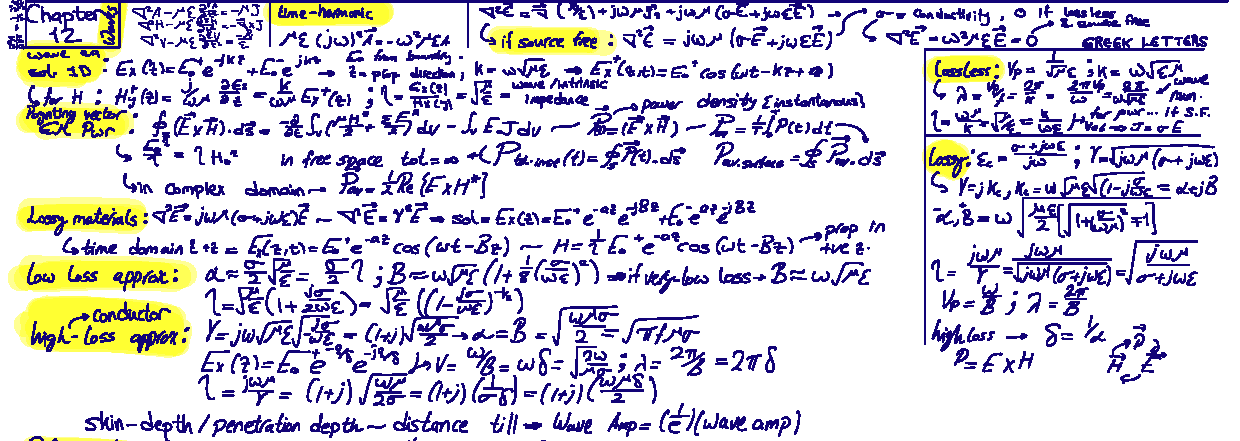
\includegraphics{pdfs/ch12fm.pdf}
\hrule
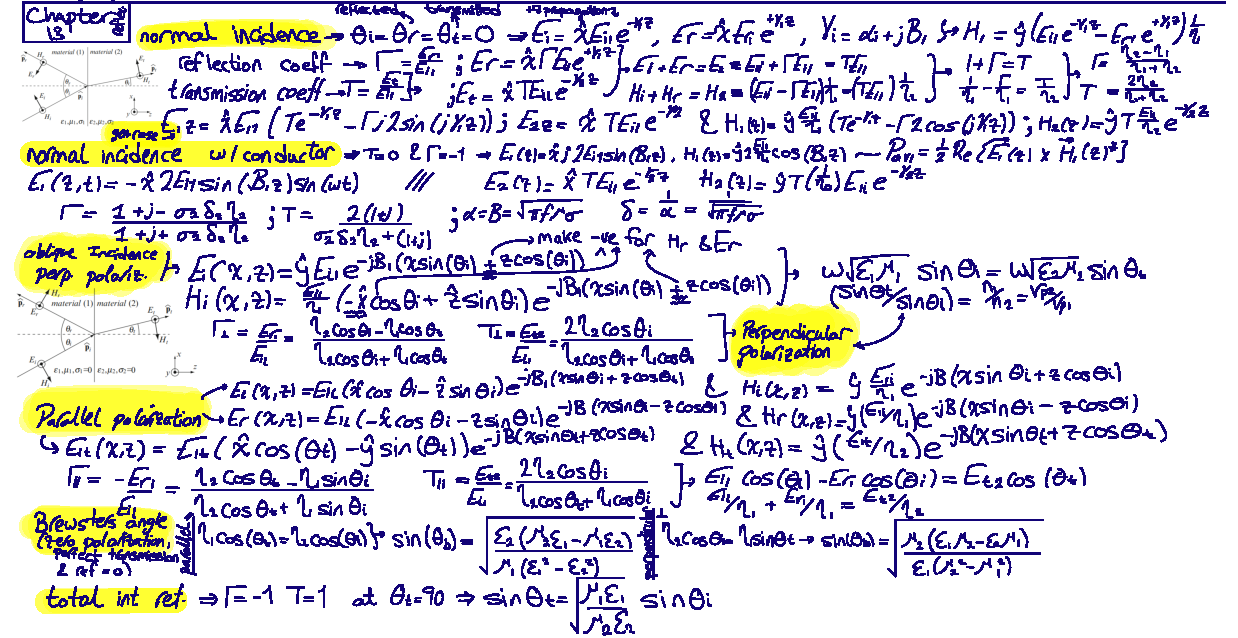
\includegraphics{pdfs/ch13fm.pdf}
\hrule

% 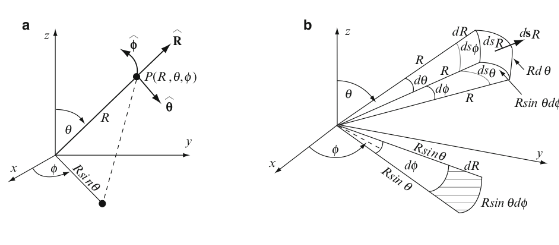
\includegraphics[scale=0.35]{images/20250113_181139.png}

\end{document}
